\paragraph{\texttt{BaseLinkButton}} \mbox{}\\

This component renders either a clickable button or a NuxtLink, depending on the props passed to it. It supports
multiple visual variants and handles both real navigation and fake/dummy behavior. The component is useful for
consistent call-to-action buttons and links across the application.

\begin{center}
    \begin{tabularx}{\textwidth}{|X|X|X|X|}
        \hline
        \textbf{Prop} & Type & Required & Description \\
        \hline
        \texttt{url} & \texttt{string} & no & The link target if used as a NuxtLink \\
        \hline
        \texttt{variant} & \texttt{number} & no & Defines the visual style (1 to 4 variants available) \\
        \hline
        \texttt{asButton} & \texttt{boolean} & no & Forces rendering as a \texttt{<button>} even if \texttt{url} is set and not \texttt{NuxtLink} \\
        \hline
        \texttt{disabled} & \texttt{boolean} & no & Disables the button (only effective when \texttt{asButton} is \texttt{true}) \\
        \hline
    \end{tabularx}
\end{center}

\paragraph{Emits}
\begin{itemize}
    \item \texttt{click} – Emitted when the button is clicked (only if rendered as a \texttt{<button>})
\end{itemize}

Moreover, both versions (the \texttt{<button>} and the \texttt{NuxtLink}) include a default slot to embed custom HTML content.



\begin{figure}[H]
    \centering
    \begin{minipage}[b]{0.32\textwidth}
        \centering
        
\includegraphics[width=\textwidth]{asset/firstButton}
    \end{minipage}
    \hfill
    \begin{minipage}[b]{0.32\textwidth}
        \centering
        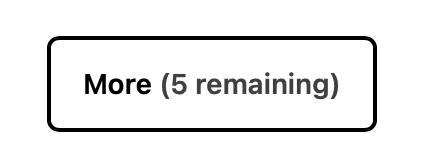
\includegraphics[width=\textwidth]{asset/secondButton}
    \end{minipage}
    \hfill
    \begin{minipage}[b]{0.32\textwidth}
        \centering
        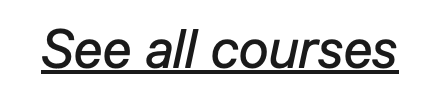
\includegraphics[width=\textwidth]{asset/thirdButton}
    \end{minipage}
    \caption{\texttt{All the buttons (Primary - Secondary - Third)}}
\end{figure}

